\chapter{Konzept}
% ================ Einstellungen =======================
\thispagestyle{fancy} \rhead{\slshape Konzept}
% ======================================================
\section{Blockschema}
\begin{figure}[H]
\centering
\includegraphics[width=\textwidth]{Bilder/p4_flowchart.png}
\caption{Blockschema}
\label{fig:flowchart}
\end{figure}
\vspace*{-0.6cm}
\newpage
\paragraph*{Aufbereitung:}
Beim Eintritt in das Museum wird das Dojo individuell angepasst. Dafür werden vom PC aus die Audiofiles mit einer dazugehörigen Korrespondenztabelle\footnote{enthält die Zuordnungen der ID. Nummern der BT-Beacons mit den Audiofiles } auf das Dojo geladen. Dabei werden die Audiofiles direkt auf der $\mu$SD-Karte und die Tabelle auf dem internen EEPROM des Mikrocontrollers gespeichert. Wenn der Switch-Block eine Spannung detektiert (Signalpfad vom USB-Switch aus), soll der Datenpfad über die Bridge geschalten sein, damit die $\mu$SD-Karte direkt als Speichermedium auf dem PC angezeigt wird. So kann das Dojo von der PC Software direkt verwaltet und angepasst werden. Ansonsten ist die $\mu$SD-Karte mit dem Audioboard verbunden, damit dieses die Audiofiles abspielen kann.
\paragraph*{Benutzung:}
Wenn der Besucher in die Nähe eines Kunstobjektes kommt, soll über das Bluetoothmodul dessen BT-Beacon erfasst werden. In der Firmware des Mikrocontrollers wird über die stärke der Signalleistung des BT-Beacons verifiziert, ob das Objekt nahe genug, oder welches näher ist. Über den Vibrationsmotor und den LEDs wird dann dem Besucher mitgeteilt, dass hier abrufbare Information ist. Gleichermassen wird auch die Zutrittskontrolle erfolgen, indem die empfangenen ID. Nummern der BT-Beacons mit den abgespeicherten abgeglichen werden. Die Objekte können über den Like-Button geliked werden, wodurch die unique ID. Nummer des BT-Beacons im internen EEPROM abgespeichert wird.
\paragraph*{Abgabe:}
Am Schluss können die im int. EEPROM gespeicherten Likes ausgewertet und eine Broschüre mit den Präferenzen des Besuchers zusammengestellt werden.
%%%%%%%%%%%%%%%%%%%%%%%%%%%%%%%%%%%%%%%%%%%%%%%%%%%%%%%%%%%%%%%%%%%%%%%%%%
\section{Hardware}
\subsection{BT-Beacon}
Diese kleinen Geräte können an den Ausstellungsstücken als Signalgeber im Museum angebracht werden. Für dieses Projekt wird ein Minew E7 Bluetooth Beacon verwendet, da dieser Beacon über die zwei bekanntesten Protokolle iBeacon und Eddystone verfügt. In der zugehörigen kostenlosen Konfigurations-App kann eingestellt werden, welches Protokoll gesendet wird. Der Beacon kann auch beide Protokolle gleichzeitig senden, bei Bedarf mit unterschiedlichen Signalstärken und Sendeintervallen. Ausserdem hat dieser Beacon eine Reichweite von 100m, ist wasserfest und verfügt sogar über einen Temperatursensor.
\newpage
\begin{landscape}
\subsection{Bluetoothmodul}
\begin{table}[H]
\begin{tabular}{|l|lll|}
\hline 
\textbf{Spezifikationen} & \textbf{HM-11 BLE} & \textbf{ISP1507 } & \textbf{SESUB-PAN-T2541} \\ 
\hline 
Version/Klasse & V4.0 BLE  & V5.0 BLE & V4.0 BLE \\ 
\hline 
Reichweite & max. 30m & max 100m & max 10m \\ 
\hline 
Sendeleistung & 23-6 dbm & max 4 dbm & 0 dbm \\ 
\hline 
Unterstützung AT Kommandos & Ja & unbekannt & Ja \\ 
\hline 
Master / Slave & Beide & Beide & Beide \\ 
\hline 
Versorgungsspannung & 3.3 V DC & 1.7 V to 3.6 V DC & 2 V to 3.6 V DC \\ 
\hline 
Kommunikationsprotokoll & UART  & UART, SPI, I2C, PDM & I2C, SPI, UART \\ 
\hline 
Äussere Abmessungen & (13.5 x 18.5 x 2.3) mm & (8 x 8 x 1) mm & (4.6 x 5.6 x 1) mm \\ 
\hline 
Preis & 11.80 CHF & 13.20 CHF & 259.30 CHF \\ 
\hline 
\end{tabular} 
\end{table}
Da Beacons in kurzen, regelmässigen Abständen im 2.4 GHz Band eine Unique ID senden, benö-
tigt das stabförmige Informations-Gerät ein Bluetooth-Modul mit UART-Schnittstelle, um diese
Information zu empfangen. 
Für den Prototyp wurden drei Bluetooth-Module tabellarisch verglichen, um eine präzise Auswahl zu treffen. Auch wenn das HM-11 BLE Bluetooth-Modul die grössten Dimensionen hat, punktet es mit der Reichweite, der Unterstützung der AT Kommandos sowie dem günstigen Preis. 
\end{landscape}
\subsection{ICSP-Header}
\begin{wrapfigure}{r}{0.3\textwidth}
	\vspace{-40pt}
  	\begin{center}
		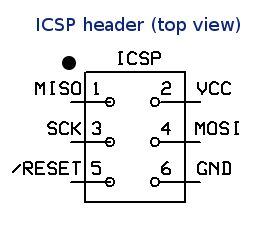
\includegraphics[scale=0.6]{Bilder/icsp_header.png}
  	\end{center}
 	\vspace{-20pt}	
	\caption{ICSP-Header}
  	\vspace{-2cm}
	\label{fig:icsp_header_topview}
\end{wrapfigure}
Damit die Firmware auf dem Dojo bearbeitbar bleibt, wird ein ICSP\footnote{In-Circuit-Serial-Programming}-Header verwendet (oder auch ISP\footnote{In-System-Programming}) \cite{ispwiki}. Damit besteht die Möglichkeit, den Mikrocontroller nach der Installation in das komplette System des Dojos programmierbar zu halten. Über eine SPI-Kommunikationsschnittstelle wird der ICSP-Header an den Mikrocontroller angeschlossen. In der Abbildung \ref{fig:icsp_header_topview} sind die Pinanschlüsse eines sechspoligen ICSP-Headers zu sehen.\\
\vspace{1cm}
\subsection{Audioboard}
Das Audioboard beinhaltet den WTV020SD-20S Audiochip. Dieser ist ein kleiner und einfacher IC für die Wiedergabe von Audiofiles. Nach Datenblatt sind mehrere unterschiedliche \textit{Modes} möglich, wobei für das Dojo der \textbf{two line serial mode} verwendet wird. Somit kann der WTV020SD Chip über den Mikrocontroller gesteuert werden und dann Audiofiles, egal welcher Adresse auf der $\mu$SD-Karte abspielen. Der Audiochip ist kompatibel für $\mu$SD-Karten mit Speicherkapazitäten bis zu 1GB. 
\subsection{Audiooutput}
Hierfür wird ein Knochenleiter (Bone conductor) verwendet. Dieser übermittelt das Audiosignal über Körperschall des Schädelknochens an das Gehör weiter.
\subsubsection{Knochenleiter}
Der Knochenleiter\footnote{den von den Dozenten zur verfügung gestellten Knochenleiter} wurde an eine Schaltung mit dem Miniverstärker LM386 angeschlossen, um dessen Verbrauch zu messen. Die Lautstärke wurde als Referenz über einen Laptop geregelt, wobei bei einer Lautstärkeneinstellung von 60 Prozent eine maximale Scheinleistung von 0.263VA und einen Effektivstrom von 0.195A erreicht wurde. Bei dieser Lautstärke ist es für eine klare Audio-Übertragung ausreichend. Für den Energieverbrauch wird mit 0.3W und im worst case Szenario mit 0.5W gerechnet.
\newpage
\subsection{$\mu$SD-Karte}
Als externes Speichermedium wird eine $\mu$SD-Karte mit einer Speicherkapazität von 1GB verwendet.
\subsubsection{Laufzeit}
Die Qualität der Audiofiles soll ungefähr in CD-Qualität erfolgen. Daraus errechnet sich nach \ref{equ:datenrate} eine Datenrate von 705.6kBit/s bei einer Bitauflösung (\textit{resolution}) von 16Bit, einer Samplefrequenz (\textit{samplerate}) von 44.1kHz und einem Kanal (\textit{channels}$\rightarrow$mono).
\begin{equation}
resolution * sample rate * channels = data rate\;[Bit/s]
\label{equ:datenrate}
\end{equation}
Daraus resultiert eine relativ hohe Qualität, welche je nach Aufnahme vom \textbf{Benutzer} angepasst werden kann. Zum Beispiel könnte die \textit{resolution} auf 8Bit, oder auch die samplerate bei der Aufnahme der Audiofiles reduziert werden. Unkomprimiert im \textit{.wav}-Format würde sich mit den 705.6kBit/s bei 1GB Speicherkapazität eine Laufzeit von \textbf{11'337.9 Sekunden} ergeben (ca. 3 Stunden 9 Minuten).
\\[0.5cm]
Nun kann die Bandbreite der Daten noch komprimiert werden. Dies kann anhand der Ansprüche des Benutzers variieren, jedoch leidet dann die Qualität. Um annähernd CD-Qualität beizubehalten, kann im \textit{.mp3}-Format die Datenrate auf 192kBit/s komprimiert werden \cite{koepenick.netkeineAngaben}. Dies entspricht einer Einsparung von 72.8\% und erhöht die Laufzeit auf \textbf{41'666.7 Sekunden} (ca. 11 Stunden 34 Minuten), was für genügend Informationen eines Museumsbesuch ausreichen sollte\footnote{diese Angaben variieren je nachdem wie der Benutzer die Audiofiles abspeichert! Dies sind nur Richtwerte.}.
\subsection{Tasten}
Für den Nutzer steht auf dem Dojo ein Tastenfeld zur Verfügung:\\
\begin{itemize}
	\item Play/Pause
	\item Volume up/down
	\item Like
	\item Vibro on/off
	\item Power on/off\\
\end{itemize}
\newpage
\subsection{Energieversorgung}
Das Dojo soll durch einen Li-Ion-Akku mit Energie versorgt werden. Die Akkulaufzeit muss die Dauer mindestens eines Museumrundgangs mit entsprechender Nutzung abdecken, wünschenswert ist eine Akkulaufzeit für einen ganzen Museumstag. Ausserdem wird eine USB-Schnittstelle (Typ C) zur Verfügung stehen, um den Akku nach Rückgabe und Auswertung des Dojos wieder aufzuladen. 
\subsubsection{Akku}
Im Handel sind Akkus vom Typ LI14500 mit einem Durchmesser von 14 mm und einer Länge von 50 mm erhältlich. Die Kapazität beträgt meist um 3 Wh, was nach ersten Abschätzungen für die gewünschte Betriebsdauer ausreicht. Die Kriterien für die Auswahl eines Akkus in der Reihenfolge ihrer Gewichtung sind: Kapazität, Zyklenfestigkeit, Schnellladefähigkeit (nur falls die Kapazität nicht für einen gesamten Tag ausreicht) und Preis. 
\subsubsection{Ladung}
Die Energie kommt über den USB-Anschluss in das Dojo. Da der Strom beim USB-Anschluss standardmässig auf 100 mA begrenzt ist, wird das Dojo mit der entsprechenden Kommunikations-Einheit ausgerüstet, um potentiell leistungsfähigeren USB-Stromquellen bis zu 1.5 A zu entlocken. Die Ladung kann über jeden beliebigen USB-C-Anschluss erfolgen. Um die Ladeinfrastruktur im Museum aufgeräumt und übersichtlich zu halten, ist eine Dockingstation vorgesehen, welche bis zu 50 Dojos aufnehmen kann. 
\section{Software}
\subsection{Software Mikrocontroller}
Der Mikrocontroller steuert das Audioboard, das BT-Modul, die Status LEDs und den Vibrationsmotor.\\[0.5cm]
Der Prototyp benutzt ein Arduino UNO-Board, für das fertige Produkt wird der Mikrocontroller des Arduino UNO's auf einen custom Print gesteckt.
\\[0.5cm]
Für jeden Besucher wird über eine serielle Schnittstelle ein Profil geladen, das beschreibt, welche Audiodatei zu welchem BT-Beacon gehört. \\
Während dem Besuch steuert der Mikrocontroller, welche Datei abgespielt werden soll, je nach dem, bei welchem Beacon der Besucher steht.\\
Zudem speichert der Mikrocontroller, welche Beacons geliked wurden und nach dem Besuch können die gespeicherten Likes wieder über die serielle Schnittstelle abgerufen werden.\\
\newpage
\subsubsection{Allgemeine Funktionsbeschreibung}
Bluetooth-Funktionen:
\begin{itemize}
	\item getClosestBeacon(): gibt die ID des nächsten Beacons zurück
	\item checkBeacon(id): gibt die Signalstärke des Beacons mit der gefragten ID zurück
\end{itemize}
\vspace*{0.2cm}
Audioboard-Steuerung:
\begin{itemize}
	\item playTrack(tracknumber): spielt die Audiodatei der Nummer tracknumber ab
	\item pausePlayback():
	\item resumePlayback():
	\item cancelPlayback():
\end{itemize}
\vspace*{0.2cm}
Interface-Steuerung:
\begin{itemize}
	\item requestManifest():
	\item deliverLikes():
\end{itemize}

\subsection{Software PC}
Über den PC wird das Dojo mit eine seriellen Schnittstelle verwaltet. Er hat alle Audiodateien, in den möglichen Sprachen und für alle Ausstellungen des Museums und stellt für jeden Besucher eine individuelle Korrespondenztabelle zusammen, basierend auf dessen Ticket und Sprachpräferenzen. Diese wird dann über die PC Software auf das Dojo geladen. Am Ende des Besuchs kann die Software die Likes vom Dojo für eine Zusammenstellung (z. B. Broschüre) mit den Interessen des Besuchers downloaden. Die Software wird voraussichtlich in Python programmiert.\\
\newpage
